\chapter{Braille}
%\section{Historia}
%
El sistema Braille es un m\'etodo utilizado por personas ciegas para leer y 
escribir. Fue ideado en 1821 por el franc\'es Louis Braille
Se basa en un m\'etodo de comunicaci\'on desarrollado y perfeccionado por 
Charles Barbier, en respuesta a la demanda de Napole\'on, de un c\'odigo que
los soldados pudieran usar para comunicarse en silencio y sin luz en la noche.
Se lo llam\'o Night writing. El sistema de Barbier era demasiado complejo para
los soldados de aprender, y fue rechazada por los militares. En 1821 visit\'o
el Instituto Nacional para Ciegos, en Par\'is, donde conoci\'o a \emph{Louis
Braille}\footnote{V\'ease - \url{http://es.wikipedia.org/wiki/Luis_Braille}},
qui\'en identific\'o el mayor defecto del c\'odigo: el dedo de la mano humana
no puede abarcar todo el s\'imbolo sin moverse, y as\'i no puede pasar
r\'apidamente de un s\'imbolo a otro.
Su modificaci\'on fue utilizar una celda de 6 puntos (el sistema Braille) que 
revolucion\'o la comunicaci\'on escrita de los ciegos.
Cada c\'elula (o celda) braille o car\'acter se compone de seis posiciones de 
puntos, dispuestos en un rect\'angulo que contiene dos columnas de tres puntos
cada uno. Un punto puede ser colocado en alguna de las seis posiciones para
formar sesenta y cuatro ($2^{6}$) permutaciones, incluido el arreglo de puntos
que no se coloca. Una permutaci\'on puede ser descrita nombrando las posiciones
en que se disponen los puntos: Las posiciones est\'an universalmente numerados
de 1 a 3, de arriba a abajo, a la izquierda, y 4 a 6, de arriba a abajo, a la
derecha como se muestra en la figura \ref{fig:braille_cell}.


% http://es.wikipedia.org/wiki/Archivo:Brailleschrift_06_KMJ.svg
\begin{figure}
\centering
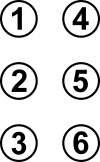
\includegraphics[scale=1]{./img/braille_cell.png}
\caption{Celda braille.}
\label{fig:braille_cell}
\end{figure}


Las l\'ineas horizontales de texto en Braille est\'an separados por un espacio
a fin de que los puntos de una l\'inea puede ser diferenciada de la de texto
en braille por encima y por debajo. La puntuacion est\'a representada por su
propio conjunto de caracteres \'unico. No existe una estandarizaci\'on
rigurosa para las distancias o medidas entre los puntos de las celdas braille,
aunque si se ha generado un estandar impl\'icito como muestra la figura
\ref{fig:distance_dots_braille}.

% http://www.wikilearning.com/monografia/abcsound-marco_teorico_1_parte/5508-9
\begin{figure}
\centering
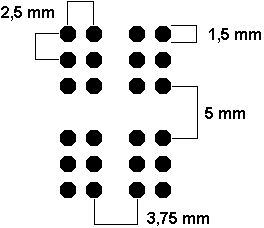
\includegraphics[scale=1]{./img/distance_dots_braille.png}
\caption{Medidas de las celdas braille.}
\label{fig:distance_dots_braille}
\end{figure}

La combinaci\'on de estos puntos generan el alfabeto braille y todos los
simbolos, como se muestra en la tabla \ref{tab:alfabeto_braille}.

\begin{table}
\begin{center}
	\enskip \enskip
	\begin{tabular}[t]{r|l}
	\hline
		\braille{a} & a 1 \\
		\braille{b} & b 2 \\
		\braille{c} & c 3 \\
		\braille{d} & d 4 \\
		\braille{e} & e 5 \\
		\braille{f} & f 6 \\
		\braille{g} & g 7 \\
		\braille{h} & h 8 \\
		\braille{i} & i 9 \\
		\braille{j} & j 0 \\
		\braille{k} & k \\
		\braille{l} & l \\
		\braille{m} & m \\
	\hline
	\end{tabular}
	\enskip \enskip
	\enskip \enskip
	\begin{tabular}[t]{r|l}
	\hline
		\braille{n} & n \\
		\braillebox{12456} & \~n \\
		\braille{o} & o \\
		\braille{p} & p \\
		\braille{q} & q \\
		\braille{r} & r \\
		\braille{s} & s \\
		\braille{t} & t \\
		\braille{u} & u \\
		\braille{v} & v \\
		\braille{w} & w \\
		\braille{x} & x \\
		\braille{y} & y \\
		\braille{z} & z \\
	\hline
	\end{tabular}
	\enskip \enskip
	\enskip \enskip
	\begin{tabular}[t]{r|l}
	\hline
		\braillebox{12356} & \'a \\
		\braillebox{2346} & \'e \\
		\braillebox{34} & \'i \\
		\braillebox{346} & \'o \\
		\braillebox{23456} & \'u \\
		\braille{,} & , \\
		\braille{;} & ; \\
		\braille{:} & : \\
		\braillebox{3} & . \\
		\braille{!} & ! \\
		\braillebox{126} & ( \\
		\braillebox{345} & ) \\
		\braillebox{35} & *	\\
		\braillebox{25} & ?	\\
		\braillebox{236} & '' \\
	\hline
	\end{tabular}
	\enskip \enskip
\end{center}
\caption{Alfabeto castellano braille.}
\label{tab:alfabeto_braille}
\end{table}



